%%%%%%%%%%%%%%%%%%%%%%%%
%%%%%   Präambel   %%%%%
%%%%%%%%%%%%%%%%%%%%%%%%

\documentclass[a4paper,
12pt,
oneside]
{article}

%%% Imports %%%

% Deutscher (und englischer) Zeichensatz
\usepackage[utf8]{inputenc}
\usepackage[english, ngerman]{babel} % Englisch als Sekundärsprache

% Schriftart Helvetica
\usepackage[scaled]{helvet}
\usepackage[T1]{fontenc}%Fonts in westeuropäischer Codierung (vor allem Sonderzeichen)

% Seitenränder
\usepackage[left=4cm,
right=2cm,
top=4cm,
bottom=2cm]
{geometry}

% Zeilenabstände
\usepackage{setspace}

% Kopf- & Fußzeile
%\usepackage{fancyhdr}

% Schriftgröße & Abstände der Überschriften anpassen
\usepackage{sectsty}
\usepackage{titlesec}

% Grafiken
\usepackage{graphicx}
\usepackage{wrapfig}

% Abkürzungsverzeichnis
\usepackage{acronym}

% Links
\usepackage[hyphens]{url}
\usepackage{etoolbox}



%%% Meta-Daten %%%
\author{David Bährens}
\title{Portfolio Nr. 6 - Überprüfung und Verarbeitung eines String mit ASP.Net}



%%% Befehle neu definieren %%%
\renewcommand\familydefault{\sfdefault} % Helvetica einbinden
% \indivskip erzeugt einen 6pt großen Zeilenabstand nach einem Absatz %
\newcommand{\sPar}{\par\vspace*{6pt}}




%%% Formatierung %%%
\onehalfspacing

% Links
\urlstyle{same}
\appto\UrlBreaks{\do\a\do\b\do\c\do\d\do\e\do\f\do\g\do\h\do\i\do\j
	\do\k\do\l\do\m\do\n\do\o\do\p\do\q\do\r\do\s\do\t\do\u\do\v\do\w
	\do\x\do\y\do\z}



%%% Kopf- & Fußzeile %%%
\pagestyle{myheadings}



%%% Literaturverzeichnis %%%
\makeatletter
\renewcommand\@biblabel[1]{}
\makeatother





%%%%%%%%%%%%%%%%%%%%%%%%%
%%%%%   Main Part   %%%%%
%%%%%%%%%%%%%%%%%%%%%%%%%

\begin{document}
	\pagenumbering{Roman}
	\begin{titlepage}
		\begin{center}
			\textbf{\huge Portfolio Nr. 6 - Überprüfung und Verarbeitung eines String mit ASP.Net} \\ \vspace{1.5cm}
			{\LARGE Portfolio} \\ \vspace{1cm}
			{\large
				Fakultät für Wirtschaft \\
				Studiengang Wirtschaftsinformatik \\
				Studienjahrgang 2018 \\ 
				Kurs C} \\ \vspace{1cm}
			\textsc{\LARGE 
				Duale Hochschule Baden-Württemberg \\
				Villingen-Schwenningen} \\ \vspace{1.5cm}
			\large
			\begin{minipage}[t]{.48\textwidth}
				Bearbeiter: \\
				David Bährens \\
				\\
				Dualer Partner: \\
				DATEV eG \\
			\end{minipage}
			\begin{minipage}[t]{.48\textwidth}
				Betreuender Dozent: \\
				Prof. Dr. Kimmig \\
			\end{minipage}
			\\ \vspace{0.5cm}
			\begin{minipage}[t]{.48\textwidth}
				
\includegraphics[width=4cm]{img/datev.png}
			\end{minipage}
			\begin{minipage}[t]{.48\textwidth}
				
\includegraphics[width=8cm]{img/dhbw.png}
			\end{minipage}
		\end{center}
	\end{titlepage}
	\clearpage
	
	
	
	\setcounter{page}{2}
	\tableofcontents
	\clearpage
	
	
	
	\section*{Abkürzungsverzeichnis}
	\addcontentsline{toc}{section}{Abkürzungsverzeichnis}
	\begin{singlespace}
		\begin{acronym}[asdfasdfasdf]
			\acro{Abb.}{Abbildung}
			\acro{ASP}{Active Server Pages}
			\acro{FCL}{Framework Class Library}
			\acro{CLR}{Common Language Runtime}
			\acro{UI}{User Interface}
			\acro{OS}{Operating System}
			\acro{MS}{Microsoft}
			\acro{z. B.}{zum Beispiel}
			\acro{API}{Application-Programming-Interface}
			\acro{ASP}{Active Server Pages}
			\acro{REST}{Representational State Transfer}
			\acro{MVC}{Model-View-Controller}
		\end{acronym}
	\end{singlespace}
	\clearpage
	
	
	
	\addcontentsline{toc}{section}{\listfigurename}
	\listoffigures
	\clearpage
	
	
	
	\addcontentsline{toc}{section}{\listtablename}
	\listoftables
	\clearpage
	
	
	
	\pagenumbering{arabic}
	
	\section{Einleitung}
	\clearpage
	
	
	
	
	\section{Theoretische Grundlagen}
	
	\subsection{ASP.Net}
	Bei ASP.Net handelt es sich um ein serverseitiges Web-Framework zur Entwicklung von dynamischen Web-Anwendungen. ASP steht für \glqq Acrive Server Pages\grqq. Dieses ist Teil des Microsoft (MS) Softwareentwicklungs und Execution-Framework .Net. .Net dient unter Windows zur Erstellung von Anwendungsprogrammen. Dessen wesentlichen beiden Bestandteile sind zum einen die Framework Class Library (FCL) und die Common Language Runtime (CLR). FCL ist eine umfangreiche Klassenbibliothek in .Net. Sie enthält beispielsweise User Interface (UI)-, File Access- oder Netzwerk-Kommunikationsklassen. Bei CLR handelt es sich um die Laufzeitumgebung in der .Net Anwendungen ausgeführt werden. .Net Programme, beispielsweise eine C\# Anwendung, greifen nicht direkt auf das Betriebssystem (OS) zu. Stattdessen wir der Programmcode in die sogenannte  MS Intermediate Language Assemby kompiliert und dann in der CLR ausgeführt. Die CLR wiederum greift dann direkt auf das darunterliegende OS zu (siehe Abb. \ref{fig:dotnet}).\footnote{Vgl. Beasley, Robert E., .Net Basics, 2020, S. 8}
	\begin{figure}[h]
		\centering
		\caption{.Net Framework}
		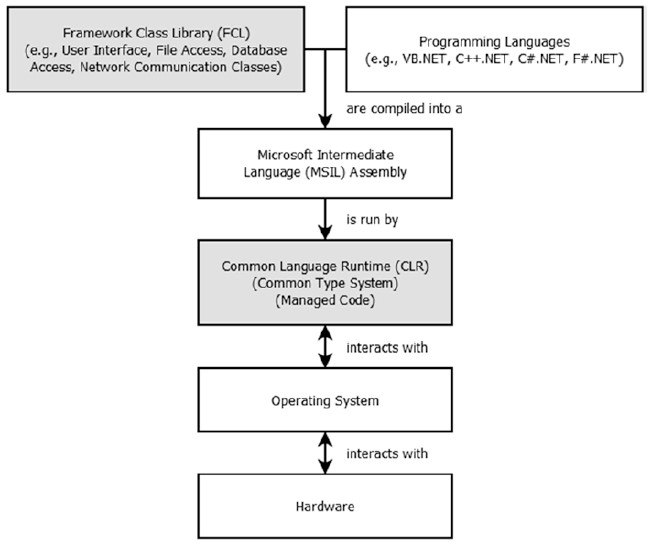
\includegraphics[width=11.5cm]{img/dotnet.jpg} \\
		\vspace{5pt}
		\footnotesize{Quelle: Beasley, Robert E., .Net Basics, 2020, S. 9}
		\label{fig:dotnet}
	\end{figure} \\
	Das .Net Framework wird jedoch fortlaufend durch .Net Core abgelöst. Hierbei handelt es sich um eine Open-Source-Plattform von MS und eine Modernisierung des .Net Frameworks. Ein besonderer Vorteil dieses moderneren Frameworks ist seine Plattformunabhängigkeit. Da ASP.Net auf .Net basiert erfolgt die Ablösung hier analog mit ASP.Net Core.\footnote{Augsten, Stephan, .Net Core, 2020} \sPar
	ASP.Net wiederum stellt verschiedene Frameworks für die Entwicklung von Web-Anwendungen zur Verfügung. Die wichtigsten sind Folgende. Zum einen gibt es das inzwischen veraltete, ereignisgesteuerte Framework \glqq Web Forms\grqq. Bei diesem wurden Oberflächen über einen Designer mit einer Drag-and-Drop Mechanik erstellt und die Logik wurde über einen Eventhandler implementiert. In der Vergangenheit kam Web Forms jedoch teilweise mit der Zustandslosigkeit des Webs in Konflikt. \\
	Ein moderneres, aktionsgesteuertes Framework stellt dagegen ASP.Net MVC dar. Dieses folgt den MVC Pattern, wodurch UI, Logik und Daten voneinander getrennt werden. MVC steht dabei für die drei wesentlichen Bestandteile in die eine MVC-Anwendung zerlegt wird, \glqq Model-View-Controller\grqq. Das Model gibt dabei die Datenstruktur, die View die Darstellung bzw. die UI und der Controller beinhaltet die Logik und verbindet das Model mit der View.\footnote{Rouse, Margaret, MVC, 2016} \\
	Dann sind da noch die Web Pages, die über die neue Razor Syntax verfügen. Razor Pages sind eine moderne Alternative zur Entwicklung von dynamischen Websites und sie stellen den Nachfolger von ASP.Net MVC dar. Sie werden in einem gesonderten Kapitel erläutert, da sie für diese Arbeit von größerer Bedeutung sind. \\
	Zuletzt ist noch ASP.Net Web API zu nennen, mit dessen Hilfe Web-Schnittstellen wie z. B. REST entwickelt werden können.\footnote{Gutsch, Jürgen, ASP.Net, 2017} \sPar
	Die .Net Entwicklung ist mit einer Reihe kompatibler Programmiersprachen möglich. Hierzu zählen beispielsweise Visual Basic, C\# oder F\#. Diese Arbeit bezieht sich im folgenden lediglich auf C\#. C\# ist eine objektorientierte und typsichere höhere Programmiersprache von MS. Ursprünglich war sie primär auf Windows ausgerichtet, inzwischen ist sie jedoch sehr universell und kann für die Entwicklung von Web-Apps eingesetzt werden.\footnote{Augsten, Stephan, C\#, 2019}
	
	\subsection{Razor Pages}
	
	\subsubsection{Allgemein}
	Razor Pages basieren auf ASP.Net MVC und zeichnen sich durch die Razor Syntax aus. Mit dieser können statische HTML Webseiten mit C\# dynamisch gemacht werden. Dies zeichnet sich dadurch aus, dass eine Webseite durch eine .cshtml Datei erstellt wird, also eine Kombination aus C\#, mittels der Razor Syntax und HTML. Razor Pages vereinen die Vorteile einer verhältnismäßig einfachen Syntax mit einem leichtgewichtigen und dennoch mächtigen Framework. Anders als ASP.Net MVC nutzen Razor Pages das Model-View-ViewModel-Pattern statt echtem MVC. Hierbei handelt es sich um eine spezielle Form der MVC-Architektur, bei der kein Controller, sondern stattdessen ein ViewModel eingesetzt wird. Dieses ist eine spezielle Implementierung eines Controllers, welcher die Logik und Programmcode hinter einer View darstellt. Jede View hat ein eigenes ViewModel, statt einem zentralen Controller, der alle Views steuert. Model und View funktionieren analog zu ihrer Funktionalität bei MVC. Die View erhält ihre benötigten Daten dabei mittels Data Binding. Analog zu MVC ist der Zweck MVVM's die Trennung von Logik, UI und Daten. Diese erfolgt bei MVVM allerdings seitenbasiert.\footnote{o. V., MVVM, 2017} Nichts desto trotz kann auch in einer Razor Page mit der MVC-Architektur gearbeitet werden falls dies gewünscht wird. \footnote{o. V., Razor Pages, 2019}
	\clearpage
	
	\subsubsection{Aufbau einer Razor Page}
	\begin{wrapfigure}{r}{7cm}
		\centering
		\caption{Aufbau Razor Pages} 
		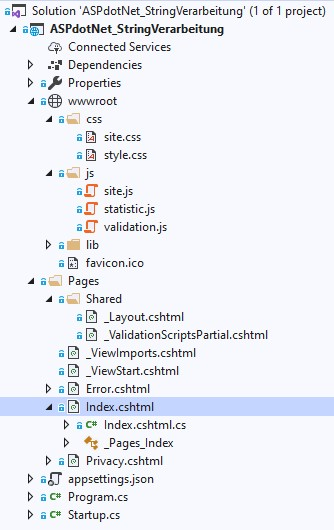
\includegraphics[width=7cm]{img/aufbau.jpg} \\
		\label{fig:aufbau}
	\end{wrapfigure}
	Ein Standard Razor Projekt besteht aus verschiedenen unterschiedlichen Dateien (siehe Abb. \ref{fig:aufbau}). Die wohl wichtigsten befinden sich in dem \glqq Page\grqq~Ordner. Dieser enthält .cshtml Dateien und .cshtml.cs Dateien, welche zusammen die eigentlichen Razor Pages darstellen. Die .cshtml Dateien sind die Views der Razor Page, allerdings könnte mit Hilfe der Razor Syntax auch Logik implementiert werden und somit jeglicher Quellcode in einer Datei gebündelt werden. Dies widerspricht allerdings dem Prinzip der Datentrennung bei MVVM und ist kein guter Programmierstil. Die .cshtml.cs dagegen sind die PageModels. Diese können sowohl die Datenstruktur, als auch die Logik beinhalten. Dies erkennt man im Übrigen auch aus der Abbildung \ref{fig:aufbau}, da hier offensichtlich kein separates Model implementiert wurde. Ein solches würde, falls benötigt, in einem separatem Model-Ordner, direkt unter dem Projekt implementiert werden. Diese sind, genau wie die PageModels, C\# Dateien. Der Startpunkt der Website bildet die Index.cshtml. Eine weitere wichtige Page-Datei ist die \_Layout.cshtml, welche ein Content Template für jede andere Page darstellt. In ihr kann z. B. der Header der Website für alle Razor Pages festgelegt werden. \\
	Offensichtlich werden Razor Pages, anders als bei ASP.Net MVC, Dateien nach dem Zweck gegliedert. Es gibt nicht nur einen Controller der die gesamte Geschäftslogik in sich vereint, sondern stattdessen gibt es viele C\# Dateien, die das ViewModel bzw. auch PageModel genannt darstellen und jeweils einer View zugeordnet sind. \\
	In wwwroot befinden sich statische Dateien, wie CSS-Style-Sheets, Bilder oder JavaScript(JS)-Dateien. Im lib Ordner wiederum befinden sich Drittanbieter-Pakete. Defaultmäßig sind dies JQuery und Bootstrap, was im Verlauf der Arbeit noch erläutert wird.
		
	\subsection{Bootstrap}
	\clearpage
	
	
	
	\section{Praxisteil: Dokumentation der Webanwendung}
	\clearpage
	
	
	
	\thispagestyle{empty}
	\nocite{*}
	\begin{thebibliography}{}
		\bibitem{.Net Basics} Beasley, Robert E., [.Net Basics] Essential ASP.NET Web Forms Development, Berkeley, CA 2020 
		
		\bibitem{.Net Core} Augsten, Stephan, [.Net Core] Definition \glqq Microsoft .NET Core Platform\grqq, Was ist .NET Core?, 09.04.2020, \url{https://www.dev-insider.de/was-ist-net-core-a-914978/} (24.05.2020)
		
		\bibitem{MVC} Rouse, Margaret, [MVC] Model View Controller (MVC), 10.2016, \url{https://www.computerweekly.com/de/definition/Model-View-Controller-MVC} (26.05.2020)
		
		\bibitem{ASP.Net} Gutsch, Jürgen, [ASP.Net] Microsofts Web-Frameworks im Vergleich, Die Qual der Wahl, 15.06.2017, \url{https://www.dotnetpro.de/frontend/qual-wahl-1226135.html} (26.05.2020)
		
		\bibitem{Csharp} Augsten, Stephan, [C\#] Definition „C-Sharp“, Was ist C\#?, 09.08.2019, \url{https://www.dev-insider.de/was-ist-c-a-846162/} (26.05.2020)
		
		\bibitem{MVVM} o. V., [MVVM] The Model-View-ViewModel Pattern, 07.08.2017, \url{https://docs.microsoft.com/de-de/xamarin/xamarin-forms/enterprise-application-patterns/mvvm} (26.05.2020)
		
		\bibitem{Razor Pages} o. V., [Razor Pages] Welcome To Learn Razor Pages \url{https://www.learnrazorpages.com/} (26.05.2020)
	\end{thebibliography}
	\addcontentsline{toc}{section}{Literatur}
	\clearpage
	
	
	\section*{Selbstständigkeitserklärung}
	\addcontentsline{toc}{section}{Selbstständigkeitserklärung}
	
\end{document}